\documentclass{article}

% Símbolos
\usepackage{recycle}
\usepackage{amsfonts}

% Teoremas y pruebas
\usepackage{amsthm}

% Figuras
\usepackage{graphicx}

% Gráficas
\usepackage{tikz}

% Cambiando "Proof" por "Demostración"
\renewcommand*{\proofname}{Demostraci\'on}

% Cambiar "Figure" por "Figura"
\renewcommand{\figurename}{Figura}

% Estilo Tikz
\tikzstyle{edge}=[shorten <=2pt, shorten >=2pt,
                  >=stealth, line width=1.1pt]
\tikzstyle{vertex}=[circle, fill=white, draw,
                    minimum size=5pt,
                    inner sep=0pt, outer sep=0pt]

% Márgenes
\addtolength{\voffset}{-1cm}
\addtolength{\hoffset}{-1.5cm}
\addtolength{\textwidth}{3cm}
\addtolength{\textheight}{2cm}

% Encabezados y Pies de Página
\usepackage{fancyhdr}
% Información del Encabezado
\lhead{Teor\'ia de Gr\'aficas II 2021-2 \\
       Tarea 1}
\rhead{Profesor: C\'esar Hern\'andez Cruz \\
       Ayudante: Daniel Garc\'ia Argueta}
% Información del Pie de Página
\rfoot{\recycle}
\cfoot{\vspace{-0.8cm}?`Realmente necesitas imprimir esta hoja?}
\lfoot{\recycle}
\pagenumbering{gobble}
\footskip = 50pt
% Línea del encabezado
\renewcommand\headrulewidth{1.5pt}
%%%%%%%%%%%%%%%%%%%%%%%%%%%%%%%%%%%%%%%%%%%%%%%%%%%%%%%%%%%%%
%%%%%%%%%%%%%%%%%%%%%%%%%%%%%%%%%%%%%%%%%%%%%%%%%%%%%%%%%%%%%
%%%%%%%%%%          Gráfica en encabezado          %%%%%%%%%%
%%%%%%%%%%%%%%%%%%%%%%%%%%%%%%%%%%%%%%%%%%%%%%%%%%%%%%%%%%%%%
%%%%%%%%%%%%%%%%%%%%%%%%%%%%%%%%%%%%%%%%%%%%%%%%%%%%%%%%%%%%%
\makeatletter
\def\headrule{{\if@fancyplain\let\headrulewidth\plainheadrulewidth\fi
\hrule\@height\headrulewidth\@width\headwidth
\vspace{0.1cm}
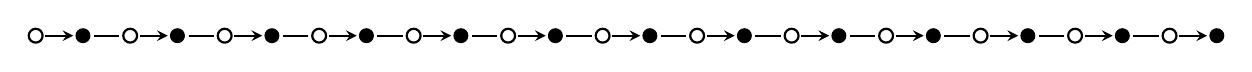
\begin{tikzpicture}
  \begin{scope}[scale=0.6]
   \foreach \x in {0,2,...,24} {
      \node [circle,draw,thick,inner sep=0,minimum size=5pt] (\x) at (\x,0){};
   }
   \foreach \x in {1,3,...,25} {
      \node [circle,draw,fill=black,inner sep=0,minimum size=5pt] (\x) at (\x,0){};
   }
   \foreach \x/\y in {0,2,...,24} {
     \pgfmathsetmacro\result{\x + 1}
     \draw [->,>=stealth,shorten <=3.5pt, shorten >=3.5pt,line width=0.7pt] (\x,0) to (\result,0);
   }
   \foreach \x/\y in {1,3,...,23} {
     \pgfmathsetmacro\result{\x + 1}
     \draw [>=stealth,shorten <=4pt, shorten >=4pt,line width=0.7pt] (\x,0) to (\result,0);
   }
   % \node [inner sep=0,minimum size=5pt] (25.5) at (25.5,-0.05){$\cdots$};
  \end{scope}
\end{tikzpicture}
\vskip-\headrulewidth
\vskip-1.5pt}}
\makeatother
%%%%%%%%%%%%%%%%%%%%%%%%%%%%%%%%%%%%%%%%%%%%%%%%%%%%%%%%%%%%%
%%%%%%%%%%%%%%%%%%%%%%%%%%%%%%%%%%%%%%%%%%%%%%%%%%%%%%%%%%%%%
%%%%%%%%%%%%%%%%%%%%%%%%%%%%%%%%%%%%%%%%%%%%%%%%%%%%%%%%%%%%%
%%%%%%%%%%%%%%%%%%%%%%%%%%%%%%%%%%%%%%%%%%%%%%%%%%%%%%%%%%%%%
%%%%%%%%%%%%%%%%%%%%%%%%%%%%%%%%%%%%%%%%%%%%%%%%%%%%%%%%%%%%%

% Estilo
\pagestyle{fancyplain}

% Macros
\newcommand{\set}[1]{\left\{ #1 \right\}}


\begin{document}

\begin{enumerate}
  \item Demuestre que si $D$ es una digr\'afica, entonces su
    condensaci\'on $D^\ast$ es ac\'iclica.

    \begin{proof}
      Sean $C_1, C_2, ..., C_n$ las componentes fuertemente
      conexas de $D$. Por definici\'on de condensaci\'on, $D^\ast$
      es la digr\'afica cuyos v\'ertices son exactamente
      $C_1, C_2, ..., C_n$ y cuyo conjunto de flechas cumple lo
      siguiente: existe una flecha de $C_i$ a $C_j$ si y solo si
      existe una flecha desde alg\'un v\'ertice de $C_i$ hacia
      alg\'un v\'ertice de $C_j$ en $D$.

      Ahora, procederemos por contradicci\'on. Supongamos que
      $D^\ast$ s\'i tiene un ciclo dirigido. Sin p\'erdida de
      generalidad, sea el ciclo $C = C_1, C_2, ..., C_k, C_1$.
      Podemos verlo en la figura~\ref{fig:cycle}.

      \begin{figure}[h]
        \centering
        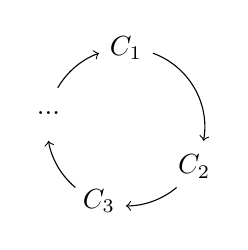
\begin{tikzpicture}[->]
          \node (i) at (90:1cm)  {$C_1$};
          \node (j) at (-30:1cm) {$C_2$};
          \node (k) at (250:1cm) {$C_3$};
          \node (l) at (170:1cm) {$...$};
          
          
          \draw (70:1cm)  arc (70:-10:1cm);
          \draw (-50:1cm) arc (-50:-90:1cm);
          \draw (230:1cm) arc (230:190:1cm);
          \draw (150:1cm) arc (150:110:1cm);
          
        \end{tikzpicture}
        \caption{Ciclo dirigido en $D^\ast$}
        \label{fig:cycle}
      \end{figure}

      Ahora, consideremos a $D'$, la subgráfica de $D$ inducida
      por el conjunto $\bigcup\limits_{i=1}^{k}C_i$. Veamos que
      $D'$ es fuertemente conexa. Para esto, consideremos
      a cualquier par de vértices $u$ y $v$ en
      $\bigcup\limits_{i=1}^{k}C_i$ y veamos que debe existir una
      trayectoria de $u$ a $v$ y otra trayectoria de $v$ a $u$.
      Primero, si ambos vértices pertenecen a la misma
      componente, entonces por definición de componente
      fuertemente conexa ya terminamos. Entonces supongamos que
      pertenecen a distintas componentes, digamos $C_u$ y $C_v$,
      respectivamente.

      Veamos que hay una trayectoria de $u$ a $v$. Es la que
      utiliza las siguientes flechas:

      \begin{itemize}
      \item Dentro de $C_u$, sigue la trayectoria desde $u$
        hasta el vértice que sale a la siguiente componente en el
        ciclo (dicha trayectoria existe porque $C_u$ es
        fuertemente conexa).
      \item De ahí, se va a la siguiente componente y al ser
        esta a su vez fuertemente conexa, puede también tomar una
        trayectoria que salga de ella y se dirija a la siguiente
        componente del ciclo.
      \item Hace esto hasta llegar a $C_v$.
      \item Una vez en $C_v$, tomamos la trayectoria hasta $v$,
        que existe por ser $C_v$ fuertemente conexa.
      \end{itemize}

      Por lo tanto, hay una trayectoria de $u$ a $v$. De manera
      análoga, hay una trayectoria de $v$ a $u$. Como $u$ y $v$
      eran vértices arbitrarios, entonces $D'$ es fuertememente
      conexa. Pero esto es una contradicción, ya que $D'$
      contiene a $C_1$, que es una componente fuertemenete
      conexa, lo que signficia que es maximal por contención.

      Por lo tanto, no puede haber un ciclo en $D^\ast$.
      
      
    \end{proof}

  \end{enumerate}
\end{document}
